% Created by tikzDevice version 0.12.6 on 2025-05-24 13:23:51
% !TEX encoding = UTF-8 Unicode
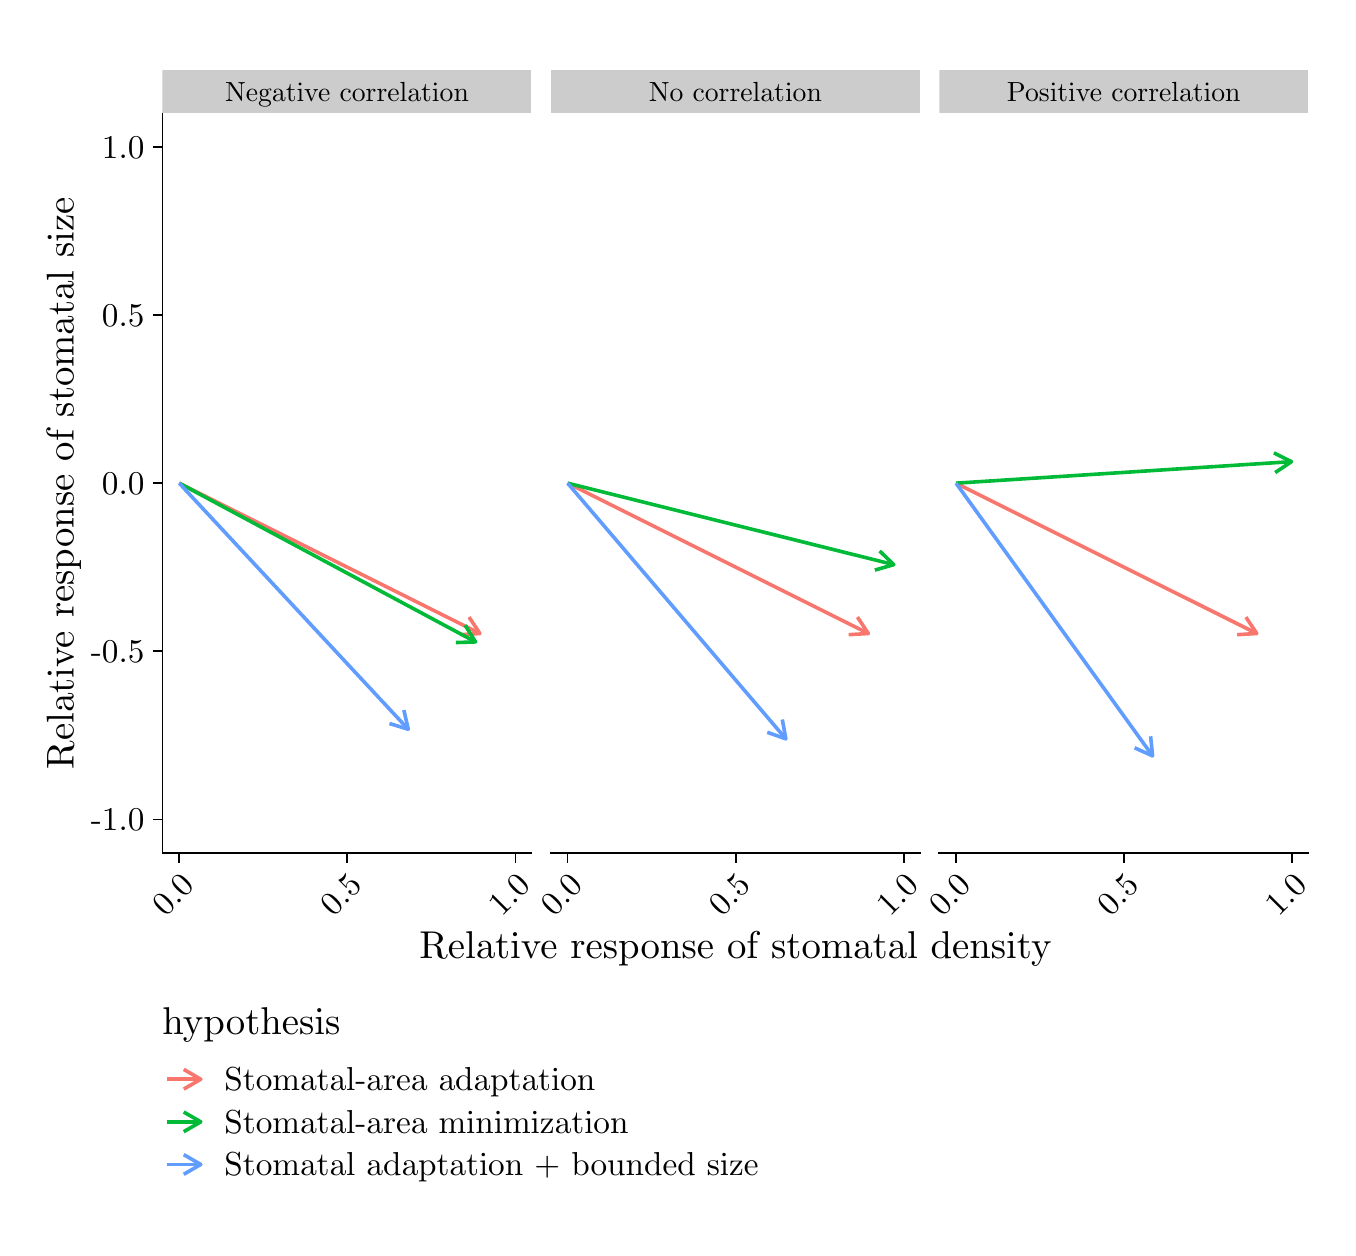
\begin{tikzpicture}[x=1pt,y=1pt]
\definecolor{fillColor}{RGB}{255,255,255}
\path[use as bounding box,fill=fillColor,fill opacity=0.00] (0,0) rectangle (469.75,433.62);
\begin{scope}
\path[clip] ( 48.69,135.40) rectangle (182.05,402.65);
\definecolor{drawColor}{RGB}{248,118,109}

\path[draw=drawColor,line width= 1.3pt,line join=round] ( 54.75,269.02) -- (163.41,214.70);

\path[draw=drawColor,line width= 1.3pt,line join=round] (156.31,214.27) --
	(163.41,214.70) --
	(159.49,220.63);
\definecolor{drawColor}{RGB}{0,186,56}

\path[draw=drawColor,line width= 1.3pt,line join=round] ( 54.75,269.02) -- (161.83,211.66);

\path[draw=drawColor,line width= 1.3pt,line join=round] (154.73,211.43) --
	(161.83,211.66) --
	(158.08,217.70);
\definecolor{drawColor}{RGB}{97,156,255}

\path[draw=drawColor,line width= 1.3pt,line join=round] ( 54.75,269.02) -- (137.52,180.10);

\path[draw=drawColor,line width= 1.3pt,line join=round] (130.72,182.19) --
	(137.52,180.10) --
	(135.93,187.04);
\end{scope}
\begin{scope}
\path[clip] (189.05,135.40) rectangle (322.40,402.65);
\definecolor{drawColor}{RGB}{248,118,109}

\path[draw=drawColor,line width= 1.3pt,line join=round] (195.11,269.02) -- (303.76,214.70);

\path[draw=drawColor,line width= 1.3pt,line join=round] (296.66,214.27) --
	(303.76,214.70) --
	(299.84,220.63);
\definecolor{drawColor}{RGB}{0,186,56}

\path[draw=drawColor,line width= 1.3pt,line join=round] (195.11,269.02) -- (312.97,239.58);

\path[draw=drawColor,line width= 1.3pt,line join=round] (306.13,237.62) --
	(312.97,239.58) --
	(307.85,244.52);
\definecolor{drawColor}{RGB}{97,156,255}

\path[draw=drawColor,line width= 1.3pt,line join=round] (195.11,269.02) -- (273.97,176.62);

\path[draw=drawColor,line width= 1.3pt,line join=round] (267.26,179.00) --
	(273.97,176.62) --
	(272.68,183.62);
\end{scope}
\begin{scope}
\path[clip] (329.40,135.40) rectangle (462.76,402.65);
\definecolor{drawColor}{RGB}{248,118,109}

\path[draw=drawColor,line width= 1.3pt,line join=round] (335.46,269.02) -- (444.12,214.70);

\path[draw=drawColor,line width= 1.3pt,line join=round] (437.02,214.27) --
	(444.12,214.70) --
	(440.20,220.63);
\definecolor{drawColor}{RGB}{0,186,56}

\path[draw=drawColor,line width= 1.3pt,line join=round] (335.46,269.02) -- (456.69,276.80);

\path[draw=drawColor,line width= 1.3pt,line join=round] (450.77,272.85) --
	(456.69,276.80) --
	(450.32,279.95);
\definecolor{drawColor}{RGB}{97,156,255}

\path[draw=drawColor,line width= 1.3pt,line join=round] (335.46,269.02) -- (406.49,170.47);

\path[draw=drawColor,line width= 1.3pt,line join=round] (400.00,173.39) --
	(406.49,170.47) --
	(405.77,177.55);
\end{scope}
\begin{scope}
\path[clip] ( 48.69,402.65) rectangle (182.05,418.48);
\definecolor{fillColor}{gray}{0.80}

\path[fill=fillColor] ( 48.69,402.65) rectangle (182.05,418.48);
\definecolor{drawColor}{RGB}{0,0,0}

\node[text=drawColor,anchor=base,inner sep=0pt, outer sep=0pt, scale=  1.00] at (115.37,407.12) {Negative correlation};
\end{scope}
\begin{scope}
\path[clip] (189.05,402.65) rectangle (322.40,418.48);
\definecolor{fillColor}{gray}{0.80}

\path[fill=fillColor] (189.05,402.65) rectangle (322.40,418.48);
\definecolor{drawColor}{RGB}{0,0,0}

\node[text=drawColor,anchor=base,inner sep=0pt, outer sep=0pt, scale=  1.00] at (255.72,407.12) {No correlation};
\end{scope}
\begin{scope}
\path[clip] (329.40,402.65) rectangle (462.76,418.48);
\definecolor{fillColor}{gray}{0.80}

\path[fill=fillColor] (329.40,402.65) rectangle (462.75,418.48);
\definecolor{drawColor}{RGB}{0,0,0}

\node[text=drawColor,anchor=base,inner sep=0pt, outer sep=0pt, scale=  1.00] at (396.08,407.12) {Positive correlation};
\end{scope}
\begin{scope}
\path[clip] (  0.00,  0.00) rectangle (469.75,433.62);
\definecolor{drawColor}{RGB}{0,0,0}

\path[draw=drawColor,line width= 0.6pt,line join=round,line cap=rect] ( 48.69,135.40) --
	(182.05,135.40);
\end{scope}
\begin{scope}
\path[clip] (  0.00,  0.00) rectangle (469.75,433.62);
\definecolor{drawColor}{RGB}{0,0,0}

\path[draw=drawColor,line width= 0.6pt,line join=round] ( 54.75,131.90) --
	( 54.75,135.40);

\path[draw=drawColor,line width= 0.6pt,line join=round] (115.49,131.90) --
	(115.49,135.40);

\path[draw=drawColor,line width= 0.6pt,line join=round] (176.23,131.90) --
	(176.23,135.40);
\end{scope}
\begin{scope}
\path[clip] (  0.00,  0.00) rectangle (469.75,433.62);
\definecolor{drawColor}{RGB}{0,0,0}

\node[text=drawColor,rotate= 45.00,anchor=base east,inner sep=0pt, outer sep=0pt, scale=  1.20] at ( 60.60,123.05) {0.0};

\node[text=drawColor,rotate= 45.00,anchor=base east,inner sep=0pt, outer sep=0pt, scale=  1.20] at (121.34,123.05) {0.5};

\node[text=drawColor,rotate= 45.00,anchor=base east,inner sep=0pt, outer sep=0pt, scale=  1.20] at (182.08,123.05) {1.0};
\end{scope}
\begin{scope}
\path[clip] (  0.00,  0.00) rectangle (469.75,433.62);
\definecolor{drawColor}{RGB}{0,0,0}

\path[draw=drawColor,line width= 0.6pt,line join=round,line cap=rect] (189.05,135.40) --
	(322.40,135.40);
\end{scope}
\begin{scope}
\path[clip] (  0.00,  0.00) rectangle (469.75,433.62);
\definecolor{drawColor}{RGB}{0,0,0}

\path[draw=drawColor,line width= 0.6pt,line join=round] (195.11,131.90) --
	(195.11,135.40);

\path[draw=drawColor,line width= 0.6pt,line join=round] (255.85,131.90) --
	(255.85,135.40);

\path[draw=drawColor,line width= 0.6pt,line join=round] (316.59,131.90) --
	(316.59,135.40);
\end{scope}
\begin{scope}
\path[clip] (  0.00,  0.00) rectangle (469.75,433.62);
\definecolor{drawColor}{RGB}{0,0,0}

\node[text=drawColor,rotate= 45.00,anchor=base east,inner sep=0pt, outer sep=0pt, scale=  1.20] at (200.95,123.05) {0.0};

\node[text=drawColor,rotate= 45.00,anchor=base east,inner sep=0pt, outer sep=0pt, scale=  1.20] at (261.69,123.05) {0.5};

\node[text=drawColor,rotate= 45.00,anchor=base east,inner sep=0pt, outer sep=0pt, scale=  1.20] at (322.43,123.05) {1.0};
\end{scope}
\begin{scope}
\path[clip] (  0.00,  0.00) rectangle (469.75,433.62);
\definecolor{drawColor}{RGB}{0,0,0}

\path[draw=drawColor,line width= 0.6pt,line join=round,line cap=rect] (329.40,135.40) --
	(462.76,135.40);
\end{scope}
\begin{scope}
\path[clip] (  0.00,  0.00) rectangle (469.75,433.62);
\definecolor{drawColor}{RGB}{0,0,0}

\path[draw=drawColor,line width= 0.6pt,line join=round] (335.46,131.90) --
	(335.46,135.40);

\path[draw=drawColor,line width= 0.6pt,line join=round] (396.20,131.90) --
	(396.20,135.40);

\path[draw=drawColor,line width= 0.6pt,line join=round] (456.94,131.90) --
	(456.94,135.40);
\end{scope}
\begin{scope}
\path[clip] (  0.00,  0.00) rectangle (469.75,433.62);
\definecolor{drawColor}{RGB}{0,0,0}

\node[text=drawColor,rotate= 45.00,anchor=base east,inner sep=0pt, outer sep=0pt, scale=  1.20] at (341.31,123.05) {0.0};

\node[text=drawColor,rotate= 45.00,anchor=base east,inner sep=0pt, outer sep=0pt, scale=  1.20] at (402.05,123.05) {0.5};

\node[text=drawColor,rotate= 45.00,anchor=base east,inner sep=0pt, outer sep=0pt, scale=  1.20] at (462.79,123.05) {1.0};
\end{scope}
\begin{scope}
\path[clip] (  0.00,  0.00) rectangle (469.75,433.62);
\definecolor{drawColor}{RGB}{0,0,0}

\path[draw=drawColor,line width= 0.6pt,line join=round,line cap=rect] ( 48.69,135.40) --
	( 48.69,402.65);
\end{scope}
\begin{scope}
\path[clip] (  0.00,  0.00) rectangle (469.75,433.62);
\definecolor{drawColor}{RGB}{0,0,0}

\node[text=drawColor,anchor=base east,inner sep=0pt, outer sep=0pt, scale=  1.20] at ( 42.19,143.41) {-1.0};

\node[text=drawColor,anchor=base east,inner sep=0pt, outer sep=0pt, scale=  1.20] at ( 42.19,204.15) {-0.5};

\node[text=drawColor,anchor=base east,inner sep=0pt, outer sep=0pt, scale=  1.20] at ( 42.19,264.89) {0.0};

\node[text=drawColor,anchor=base east,inner sep=0pt, outer sep=0pt, scale=  1.20] at ( 42.19,325.63) {0.5};

\node[text=drawColor,anchor=base east,inner sep=0pt, outer sep=0pt, scale=  1.20] at ( 42.19,386.37) {1.0};
\end{scope}
\begin{scope}
\path[clip] (  0.00,  0.00) rectangle (469.75,433.62);
\definecolor{drawColor}{RGB}{0,0,0}

\path[draw=drawColor,line width= 0.6pt,line join=round] ( 45.19,147.54) --
	( 48.69,147.54);

\path[draw=drawColor,line width= 0.6pt,line join=round] ( 45.19,208.28) --
	( 48.69,208.28);

\path[draw=drawColor,line width= 0.6pt,line join=round] ( 45.19,269.02) --
	( 48.69,269.02);

\path[draw=drawColor,line width= 0.6pt,line join=round] ( 45.19,329.76) --
	( 48.69,329.76);

\path[draw=drawColor,line width= 0.6pt,line join=round] ( 45.19,390.50) --
	( 48.69,390.50);
\end{scope}
\begin{scope}
\path[clip] (  0.00,  0.00) rectangle (469.75,433.62);
\definecolor{drawColor}{RGB}{0,0,0}

\node[text=drawColor,anchor=base,inner sep=0pt, outer sep=0pt, scale=  1.40] at (255.72, 97.42) {Relative response of stomatal density};
\end{scope}
\begin{scope}
\path[clip] (  0.00,  0.00) rectangle (469.75,433.62);
\definecolor{drawColor}{RGB}{0,0,0}

\node[text=drawColor,rotate= 90.00,anchor=base,inner sep=0pt, outer sep=0pt, scale=  1.40] at ( 16.64,269.02) {Relative response of stomatal size};
\end{scope}
\begin{scope}
\path[clip] (  0.00,  0.00) rectangle (469.75,433.62);
\definecolor{drawColor}{RGB}{0,0,0}

\node[text=drawColor,anchor=base west,inner sep=0pt, outer sep=0pt, scale=  1.40] at ( 48.69, 69.70) {hypothesis};
\end{scope}
\begin{scope}
\path[clip] (  0.00,  0.00) rectangle (469.75,433.62);
\definecolor{drawColor}{RGB}{248,118,109}

\path[draw=drawColor,line width= 1.3pt,line join=round] ( 50.23, 53.64) -- ( 62.55, 53.64);

\path[draw=drawColor,line width= 1.3pt,line join=round] ( 56.39, 50.08) --
	( 62.55, 53.64) --
	( 56.39, 57.19);
\end{scope}
\begin{scope}
\path[clip] (  0.00,  0.00) rectangle (469.75,433.62);
\definecolor{drawColor}{RGB}{0,186,56}

\path[draw=drawColor,line width= 1.3pt,line join=round] ( 50.23, 38.24) -- ( 62.55, 38.24);

\path[draw=drawColor,line width= 1.3pt,line join=round] ( 56.39, 34.68) --
	( 62.55, 38.24) --
	( 56.39, 41.79);
\end{scope}
\begin{scope}
\path[clip] (  0.00,  0.00) rectangle (469.75,433.62);
\definecolor{drawColor}{RGB}{97,156,255}

\path[draw=drawColor,line width= 1.3pt,line join=round] ( 50.23, 22.84) -- ( 62.55, 22.84);

\path[draw=drawColor,line width= 1.3pt,line join=round] ( 56.39, 19.28) --
	( 62.55, 22.84) --
	( 56.39, 26.39);
\end{scope}
\begin{scope}
\path[clip] (  0.00,  0.00) rectangle (469.75,433.62);
\definecolor{drawColor}{RGB}{0,0,0}

\node[text=drawColor,anchor=base west,inner sep=0pt, outer sep=0pt, scale=  1.20] at ( 71.09, 49.50) {Stomatal-area adaptation};
\end{scope}
\begin{scope}
\path[clip] (  0.00,  0.00) rectangle (469.75,433.62);
\definecolor{drawColor}{RGB}{0,0,0}

\node[text=drawColor,anchor=base west,inner sep=0pt, outer sep=0pt, scale=  1.20] at ( 71.09, 34.10) {Stomatal-area minimization};
\end{scope}
\begin{scope}
\path[clip] (  0.00,  0.00) rectangle (469.75,433.62);
\definecolor{drawColor}{RGB}{0,0,0}

\node[text=drawColor,anchor=base west,inner sep=0pt, outer sep=0pt, scale=  1.20] at ( 71.09, 18.70) {Stomatal adaptation + bounded size};
\end{scope}
\end{tikzpicture}
